
\section{Reproduction of main experiment}
\label{sec:main-exp}

In this section, we present our reproduction of the main experiments from \citep{ncsn-paper}, which consist of training RefineNet models (\autoref{sec:architecture}) on MNIST, CIFAR-10 and CelebA datasets and performing sampling and inpainting with the best models. Following \cite{ncsn-paper}, the baseline was trained without annealing, conditioned on only one noise level ($\sigma=0.01$), while the final model was conditioned on a geometric sequence $\{\sigma_i\}_{i = 1}^{10}$ from 1 to 0.01. All models were trained for 200,000 iterations. 

\subsection{Image generation}

\begin{wrapfigure}{h!}{0.39\textwidth}
    \centering
    \vspace{-2mm}
    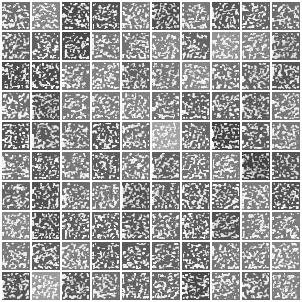
\includegraphics[scale=0.38]{figures/samples/baseline.png}
    \caption{Samples from the baseline.}
    \label{fig:baseline}
    \vspace{-2mm}
\end{wrapfigure}

\paragraph{One noise level}
The samples generated from the baseline model trained on MNIST are given in \autoref{fig:baseline}. Following \cite{ncsn-paper}, we used $T=1000$ and $\epsilon=2 \cdot 10^{-5}$ for sampling. As we can see, the model fails to generate correct samples, which is in agreement with the original results, even for a simple dataset such as MNIST. Due to limited computational resources, we omit training the baseline for CIFAR-10 and CelebA, and focus instead on additional experiments. Overall, we consider this choice of baseline redundant, as the importance of multiple noise levels has already been showcased on the toy example (\autoref{sec:repr-of-toy}). In our opinion, a more informative baseline would be a simplified network architecture or simpler annealing schedule; we will investigate this in \autoref{sec:additional}.

\paragraph{Multiple noise levels} We now present our results from replicating the main experiments with models trained with a geometric sequence $\{\sigma_i\}_{i=1}^{10}$, to showcase that this approach yields reasonable samples of real data. The loss curves are given in \autoref{fig:losses} in the Appendix. We chose the best model from checkpoints as explained in \autoref{sec:eval}. The samples obtained from this model with $T=100$ and $\epsilon=2 \cdot 10^{-5}$ and intermediate samples from each $q_{\sigma_i}$ are shown in \autoref{fig:samp}. Additional samples are provided in the Appendix. The best model for CIFAR-10 was found at 120k iterations and for CelebA at 30k. The Inception score and FID computed from 50k samples from the final model for CIFAR-10 were \bm{$6.5 \pm 0.118$} and \bm{$33.0$}, and for CelebA \bm{$3.4 \pm 0.0395$} and \bm{$81.5$}.

\begin{figure}[h!]
  \centering
     \subfloat[MNIST samples]{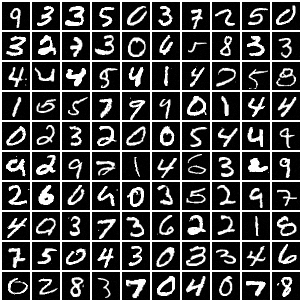
\includegraphics[width=0.31\linewidth]{figures/samples/mnist_samples.png}\label{fig:mnist-samp}}\hspace{2mm}
     \subfloat[CIFAR-10 samples]{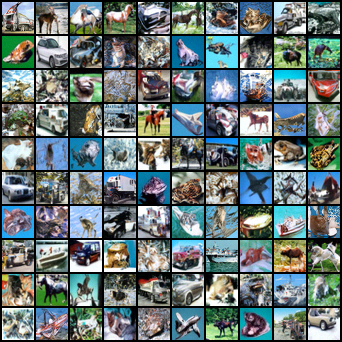
\includegraphics[width=0.31\linewidth]{figures/samples/refinenet128_cifar10_L10_step120000.png}\label{fig:cifar10-samp}}\hspace{2mm}
     \subfloat[CelebA samples]{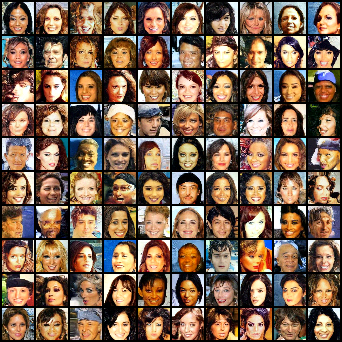
\includegraphics[width=0.31\linewidth]{figures/samples/celeba_samples.png}\label{fig:celeba-samp}} \\
     \subfloat[MNIST intermediate]{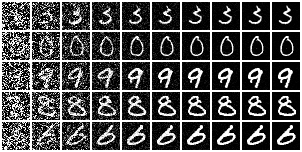
\includegraphics[width=0.31\linewidth]{figures/samples/refinenet64_mnist_L10_step200000_intermediate.png}\label{fig:mnist-intermediate}}\hspace{2mm}
     \subfloat[CIFAR-10 intermediate]{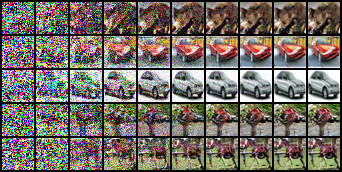
\includegraphics[width=0.31\linewidth]{figures/samples/refinenet128_cifar10_L10_step120000_intermediate.png}\label{fig:cifar10-intermediate}}\hspace{2mm}
     \subfloat[CelebA intermediate]{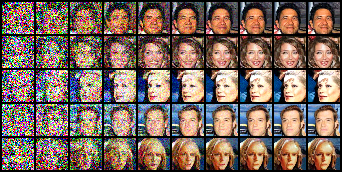
\includegraphics[width=0.31\linewidth]{figures/samples/refinenet128_celeb_a_L10_step30000_intermediate.png}\label{fig:celeba-intermediate}}
     
     \caption{Uncurated samples generated from trained models for MNIST, CIFAR-10 and CelebA datasets with annealed Langevin dynamics (a-c) and intermediate steps during sampling process (d-f).}
     \label{fig:samples}
     \vspace{-3mm}
\end{figure}

As we can see, while the samples are qualitatively good, our Inception and FID scores for CIFAR-10 are noticeably worse than those reported in the paper (8.87$\pm$.12 and 25.32, respectively). A possible reason could be the high variability in the FID score when choosing the best model as described in \autoref{sec:eval}; we show that the FID score fluctuates for checkpoints for both CIFAR-10 and CelebA in \autoref{fig:fid} in the Appendix. We believe using more samples at each checkpoint (the standard for FID is a minimum of 2048, while here we only used 1000 as per \cite{ncsn-paper}) would yield a more reliable metric, but this comes at the cost of more expensive computations. There could also be some differences in the architecture that were missed in the implementation.\footnote{We initially considered the number of residual blocks, but with 2 blocks the results did not improve.} As an extension to the original paper, we also computed FID and IS for CelebA. While cropping and resizing means that results are not directly comparable to results from literature, we can see that our achieved results are significantly worse -- the current reported state of the art FID score for $64 \times 64$ CelebA is $4.00$ \cite{DBLP:journals/corr/abs-1904-00284}, while we obtained $81.5$. Perhaps an interesting observation is that there are more female than male faces generated, which also reflects the ratio of these in the training data. In the interest of reproducability, we also report the time cost of training and sampling for each dataset in \autoref{tab:times} in the Appendix.

% \subsection{Nearest neighbours}
Following \cite{ncsn-paper}, we find $k$ nearest neighbours for a set of generated samples from the training data with respect to $l_2$ distance. Results are shown in \autoref{fig:nn}, and more extensive examples in \autoref{fig:nn-large} in the Appendix. As we can see, the network has not memorised exact training images, but still preserves some high-level features from the training set such as colour, shape, style, orientation etc.\footnote{\textbf{Disclaimer}: We implemented this before the authors added nearest-neighbour calculations to their work on 29th Oct 2019, which additionally measures distance based on activations from the Inception network.}\vspace{-4mm}

\begin{figure}[h!]
  \centering
     \subfloat[MNIST]{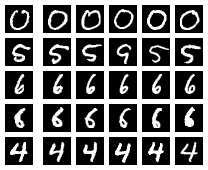
\includegraphics[width=0.28\linewidth]{figures/samples/refinenet64_mnist_L10_step200000_5nearest.png}\label{fig:mnist-nn}}\hspace{3mm}
     \subfloat[CIFAR-10]{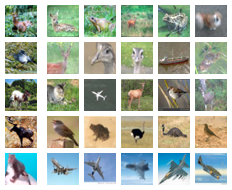
\includegraphics[width=0.28\linewidth]{figures/samples/refinenet128_cifar10_L10_step120000_5nearest.png}\label{fig:cifar10-nn}}\hspace{3mm}
     \subfloat[CelebA]{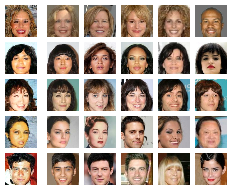
\includegraphics[width=0.28\linewidth]{figures/samples/refinenet128_celeb_a_L10_step30000_5nearest.png}\label{fig:celeba-nn}}
     \caption{$k=5$ nearest neighbours from the training data for 5 samples based on $l_2$-distance.}
     \label{fig:nn}
     \vspace{-3mm}
\end{figure}

\subsection{Inpainting}
We also performed inpainting as in \cite{ncsn-paper}, occluding the right half of the image and completing the image with annealed Langevin dynamics. The results are shown in \autoref{fig:inpainting}. As we can see, the models perform extremely well, especially in recovering the background for CIFAR-10 and the right half of the face for CelebA. Moreover, inpaintings for the same image are diverse, which showcases the generalisation capacity of the approach. Furthermore, one advantage of this method is that it is able to handle arbitrary occlusion shapes well (\autoref{fig:celeb_a_inpainting} in the Appendix). A nice addition would be to quantify the quality of results by measuring signal-to-noise ratio, but we leave this as future work.\vspace{-3mm}

\begin{figure}[h!]
  \centering
     \subfloat[MNIST]{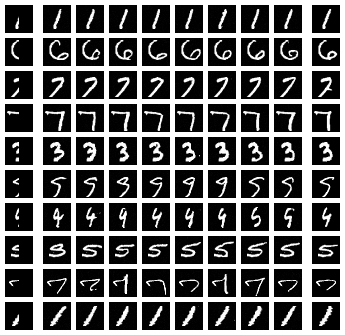
\includegraphics[width=0.311\linewidth]{figures/samples/refinenet64_mnist_L10_step200000_inpainting.png}\label{fig:mnist-inpainting}}\hspace{1mm}
     \subfloat[CIFAR-10]{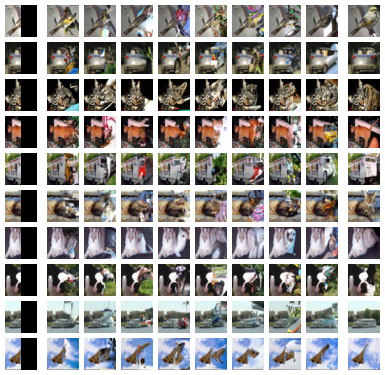
\includegraphics[width=0.311\linewidth]{figures/samples/refinenet128_cifar10_L10_step120000_inpainting.png}\label{fig:cifar10-inpainting}}\hspace{1mm}
     \subfloat[CelebA]{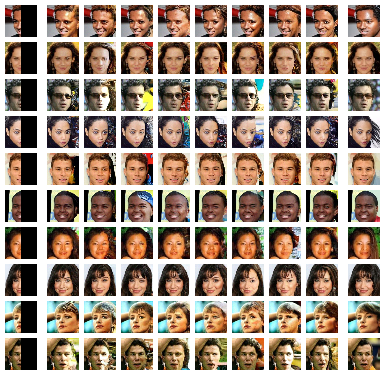
\includegraphics[width=0.311\linewidth]{figures/samples/refinenet128_celeb_a_L10_step30000_inpainting.png}\label{fig:celeba-inpainting}}
     \caption{Inpainting for occluded images from the training set. The occluded image is given in the leftmost column, and the true image in the rightmost column.}
     \label{fig:inpainting}
\end{figure}\vspace{-4mm}

